\section{Results}
\label{sec:results}

In this section we describe the results of the simulation with the potential barrier.
In the first few time steps the distribution filled the zero potential volume.
Right after filling the zero potential area, small amount of probability density penetrated deeper into the larger potential sections of the simulated volume.
This can be observed in figure~\ref{fig:penetrating_potential}.
We speculate that this is the result of high initial momentum of the distribution.
The high energy resulted in quantum tunnelling-like behaviour, where the wave was able to defeat the potential obstacle to some degree.
The amount of penetration could be related to the fact that the potential barrier increases linearly towards the edge of simulated volume.
We also considered the possibility of the penetration being simply an artifact that is the result of the heuristic initial wave.

\begin{figure}
	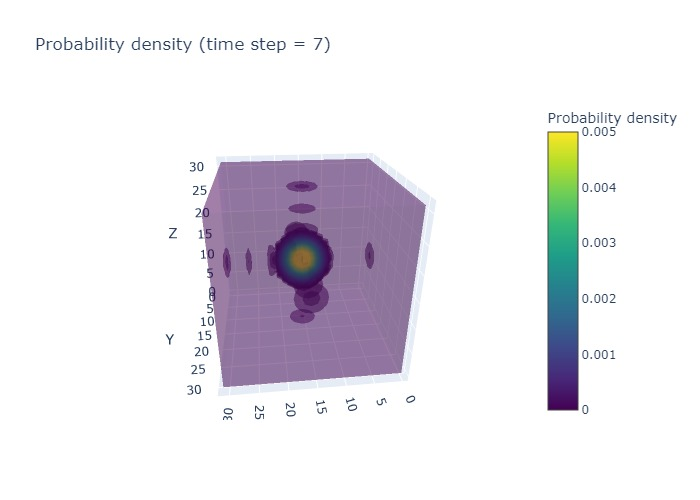
\includegraphics[width=0.75\textwidth]{"figures/probability_density007.jpeg"}
	\caption{Wave penetrating the linearly increasing potential barrier at an early stage of the simulation}
	\label{fig:penetrating_potential}
\end{figure}

After the previously described initial phase the wave function filled the middle part of the simulated volume where the potential was zero and began interfering with itself.
When the wave first filled the zero potential cube, it was seemingly homogenous observing only the probability density.
Shortly after nodes with higher probability density emerged from the homogenous volume.
These nodes where arranged in a grid-like pattern.
This can be observed in figure~\ref{fig:node_pattern}.

\begin{figure}
	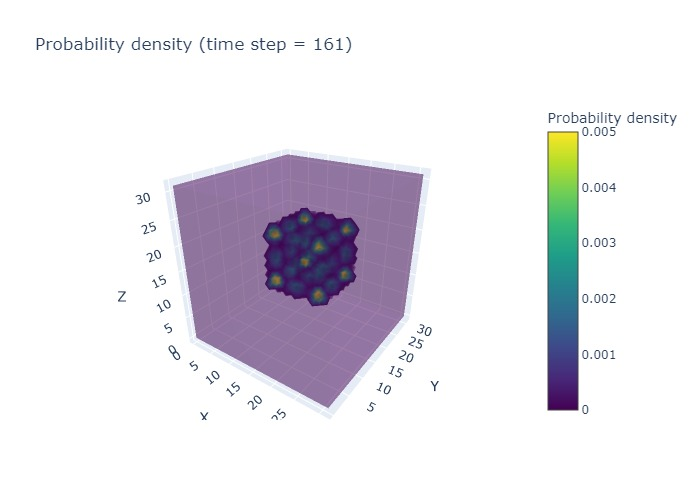
\includegraphics[width=0.75\textwidth]{"figures/probability_density161.jpeg"}
	\caption{Wave forming pattern of high probability density nodes}
	\label{fig:node_pattern}
\end{figure}

The nodes transformed into a series of different patterns.
These patterns showed periodicity.
This behaviour is similar to the phenomena called quantum revival \cite{styer2001quantum}.






